\documentclass[tikz,border=10pt]{standalone}
\usetikzlibrary{calc}
% Scale s=0.020101 cm/px, centred on (236,160) px (y flipped)
\begin{document}
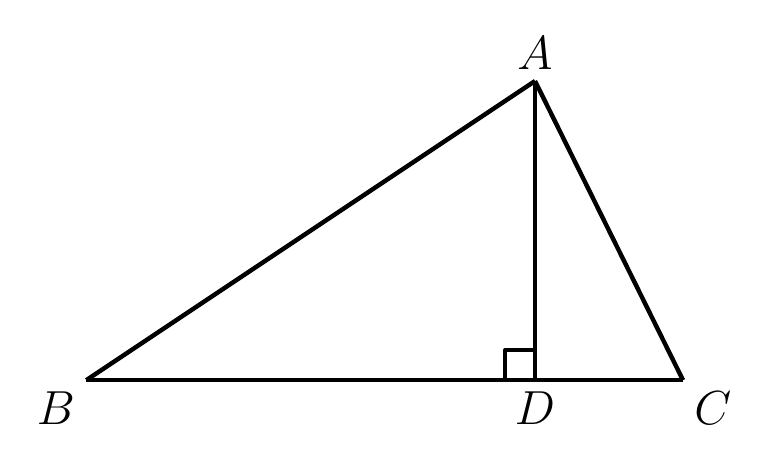
\begin{tikzpicture}[line join=round, line width=1.6pt, font=\fontsize{16.5}{19.8}\selectfont]
  % Named coordinates
  \coordinate (A) at (1.9096,1.9096);
  \coordinate (B) at (-3.7890,-1.8900);
  \coordinate (C) at (3.7890,-1.8900);
  \coordinate (D) at (1.9096,-1.8900);

  % Triangle sides
  \draw (A) -- (B);
  \draw (A) -- (C);
  \draw (B) -- (C);
  % Altitude
  \draw (A) -- (D);

  % Right-angle mark at D (inside the angle between DA and DC)
  \draw (D) ++(-0.38,0) -- ++(0,0.38) -- ++(0.38,0);

  % Labels
  \node[above] at (A) {$A$};
  \node[below left] at (B) {$B$};
  \node[below right] at (C) {$C$};
  \node[below] at (D) {$D$};
\end{tikzpicture}
\end{document}